% This document is made freely avaiable through the CC0 1.0 Universal license (logo excluded).
% Similar material avaiable at https://github.com/noahhaworth/CAD_Material
% Things to fix:
%		make wording more accurate + spelling check
%		consider adding color
%		ensure all figures are well defined

\documentclass{article}
\usepackage[utf8]{inputenc}
\usepackage[legalpaper, landscape,top=.5in,right=1.5in,left=1.5in,bottom=1.5in]{geometry}
\usepackage{ragged2e}
\usepackage{graphicx}
\usepackage{float}
\usepackage{setspace}
\usepackage[labelfont=bf]{caption}
\usepackage{hyperref}
\usepackage{array}
\usepackage{xcolor}
\hypersetup{colorlinks=true, urlcolor=blue}

\begin{document}
\definecolor{noah}{HTML}{ffffff}
\pagecolor{noah}
\center
\Huge{\textbf{SolidWorks Assembly Practice Problems}\\[3mm] \hrule
\vspace{4mm}
\includegraphics[width=0.15\textwidth]{~/Documents/github/nwh.png}\\[4mm] 
\justify\normalsize
\textbf{Information:} The following problems were originally part of a three hour SolidWorks assembly exam. An instructional video is avaiable \href{https://www.youtube.com/watch?v=o4F9eGQ8W1k&list=PL_ks8ETHwZM17sjwTXLjIJNA6Z_pSvy5g&index=4&t=3s}{here}. You are free to do as you please with this document. More material similar to this (including the .sldprts for these assemblies) can be found \href{https://github.com/noahhaworth/CAD_Material}{here}.\\[10mm]
\newpage
\newgeometry{top=.5in,right=1.5in,left=1.5in,bottom=1.5in}

%problem 1
\textbf{P1}\\[0mm]
\begin{minipage}[c]{.8\textwidth}
\begin{figure}[H]
  \centering
  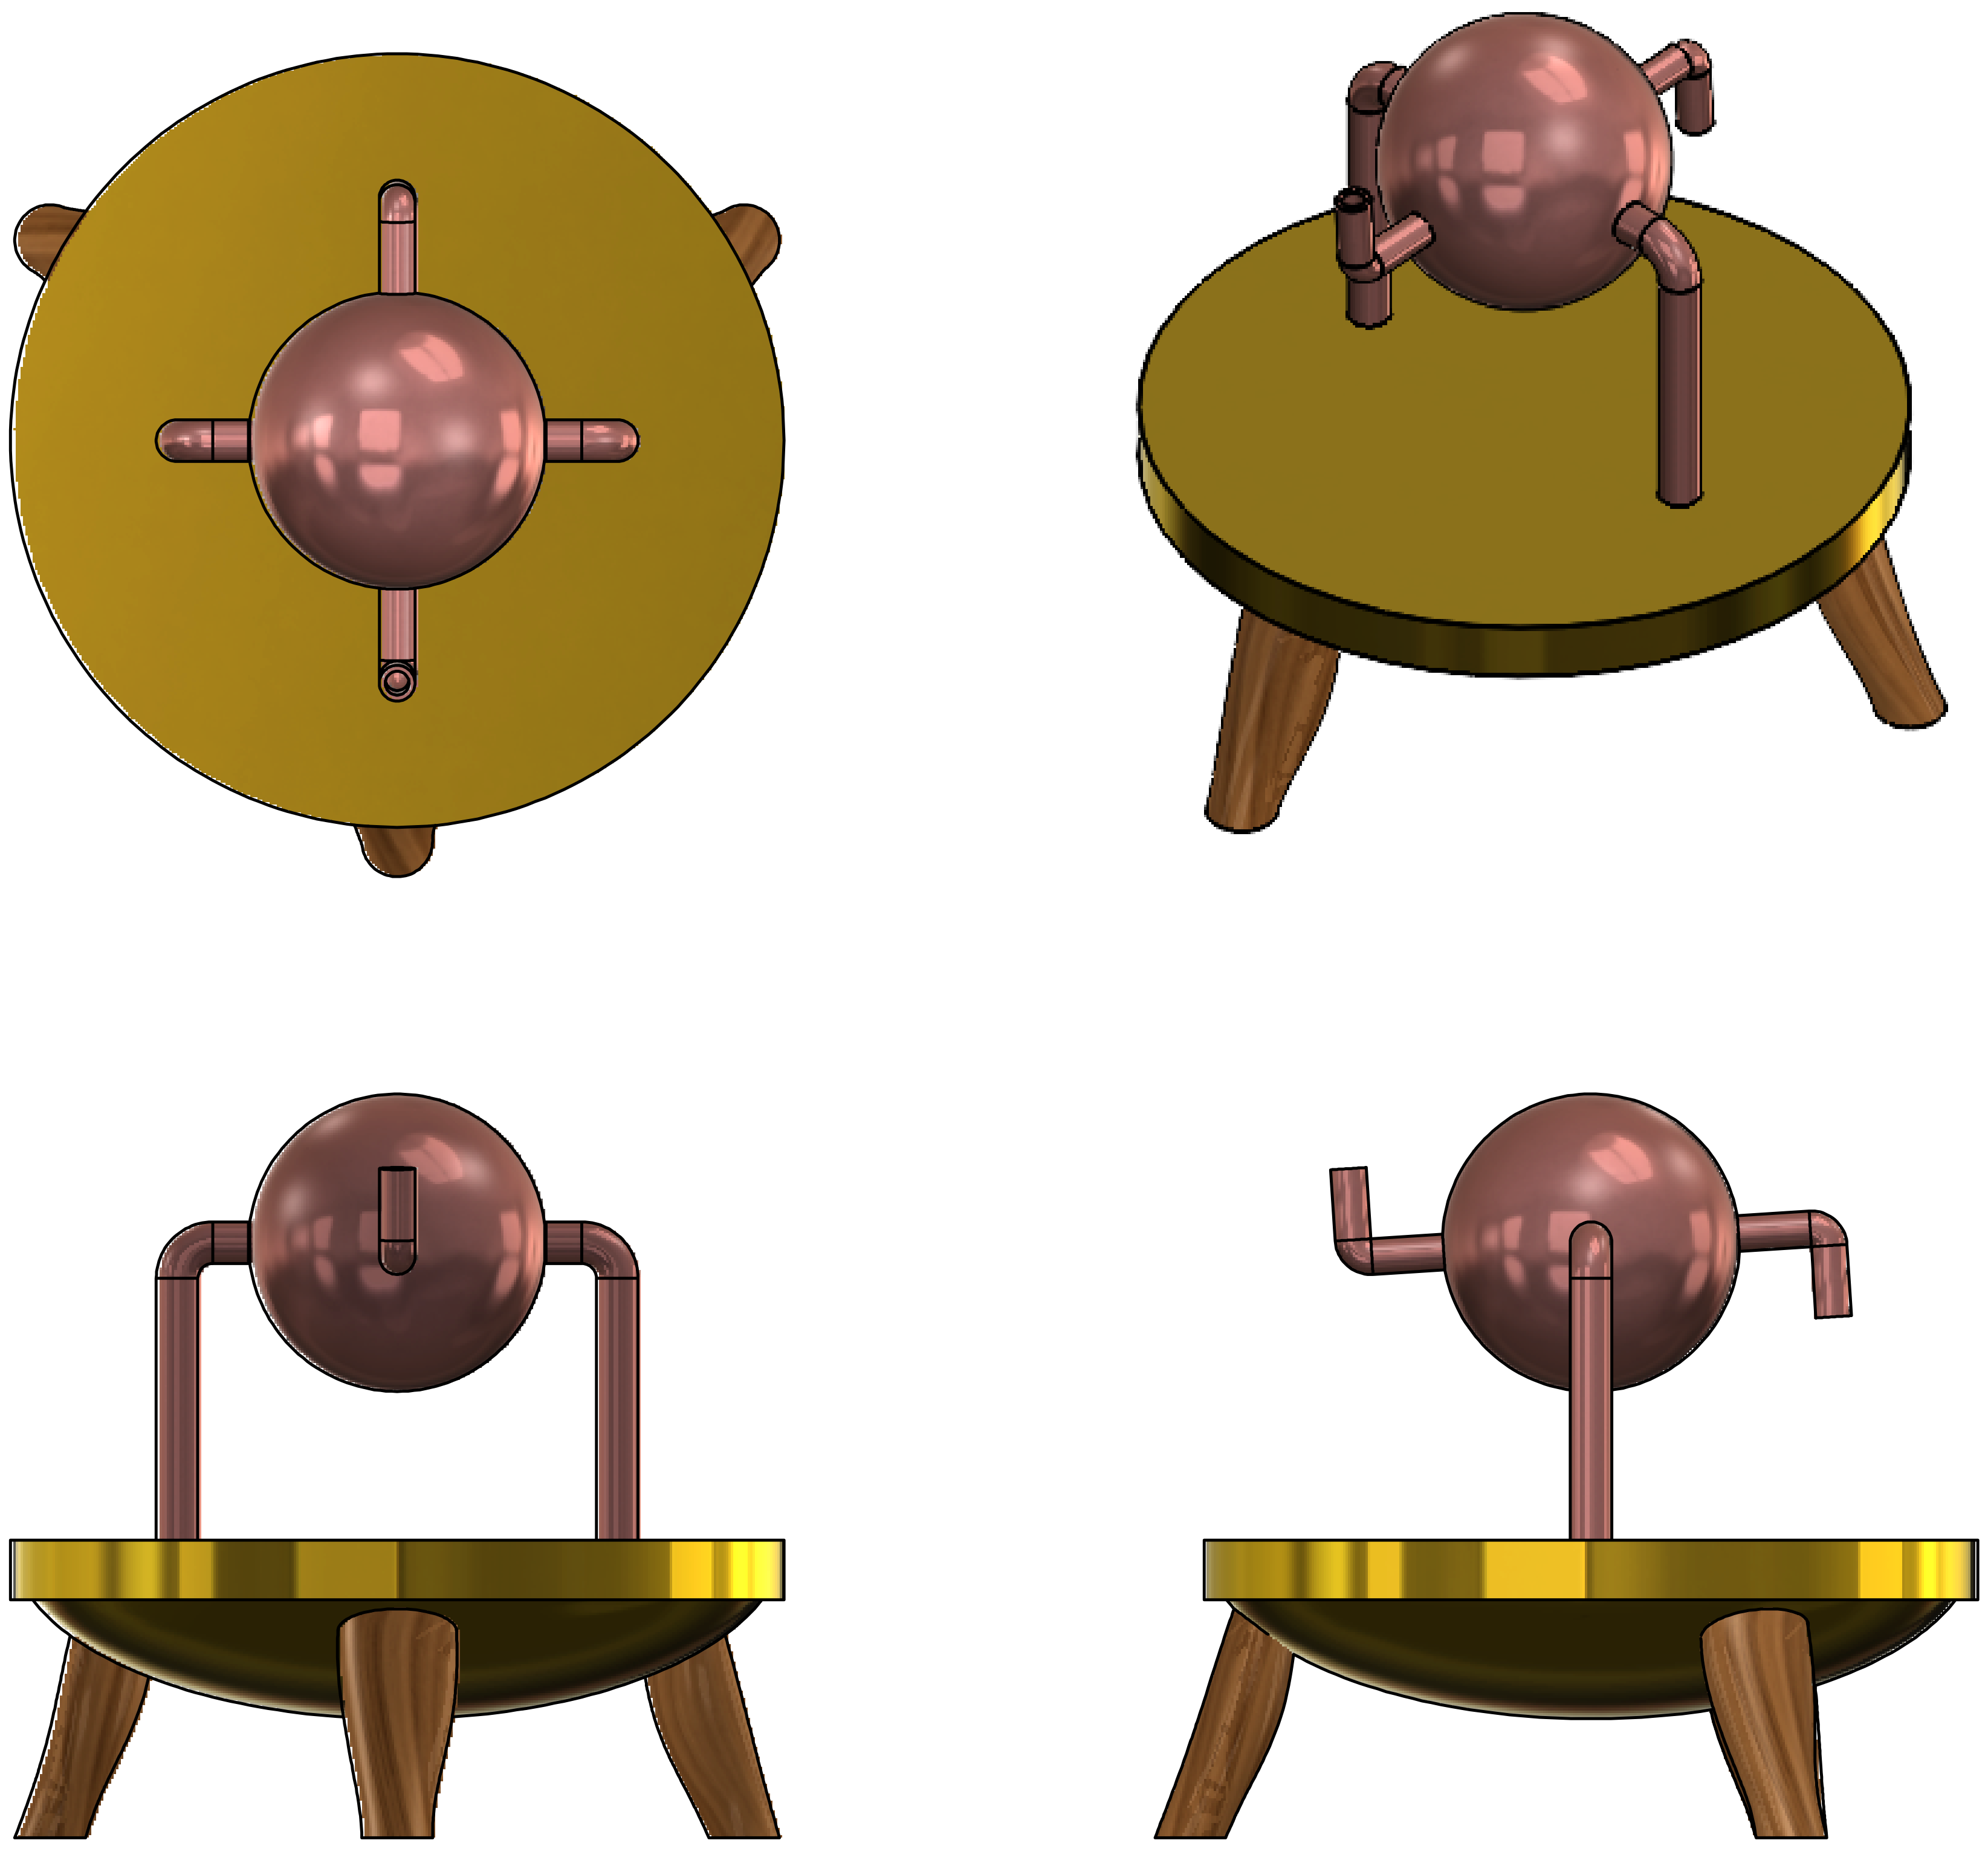
\includegraphics[width=.575\linewidth]{images/1.png}  
  \caption{Hero's Engine}
  \label{fig:1}
\end{figure}
\vspace{1mm}
\end{minipage}
\begin{minipage}[c]{.25\textwidth}
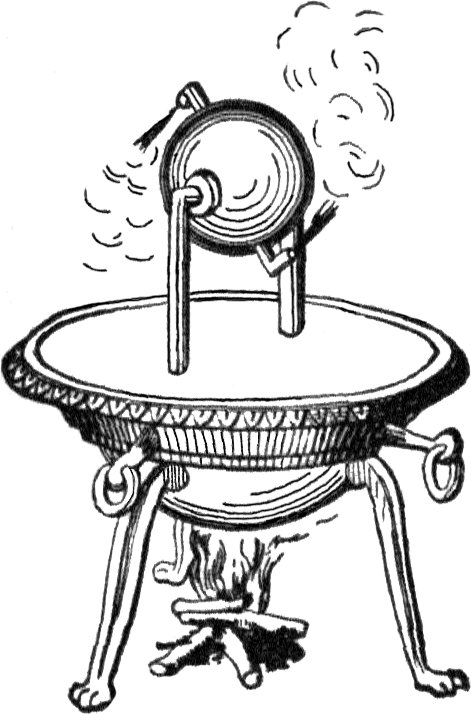
\includegraphics[width=.7\linewidth]{images/1b.png}
\end{minipage}
\noindent Aeolus is the Greek god of air and wind. Marcus Vitruvius Pollio mentioned an aeolipile (also called eolipile, or more recently Hero’s engine) in 15 B.C.E.. Not much later, Hero of Alexandria of Roman Egypt described how to make this device. This device is considered the first steam engine. Unfortunately, these devices were only seen as novelties, or party tricks. They were not used practically. One could speculate that had investigation into steam engines continued at this time, the industrial revolution would have likely started much sooner than it did. Please assemble Hero’s engine as seen in \textit{Figure 1}. There is a fundamental flaw in the specific model seen in \textit{Figure 1}. Tell me what this flaw is in a Word or txt file and you will get an extra 5 points. 

%problem 2
\textbf{P2}\\[0mm]
\begin{minipage}[c]{.75\linewidth}
\begin{figure}[H]
  \centering
  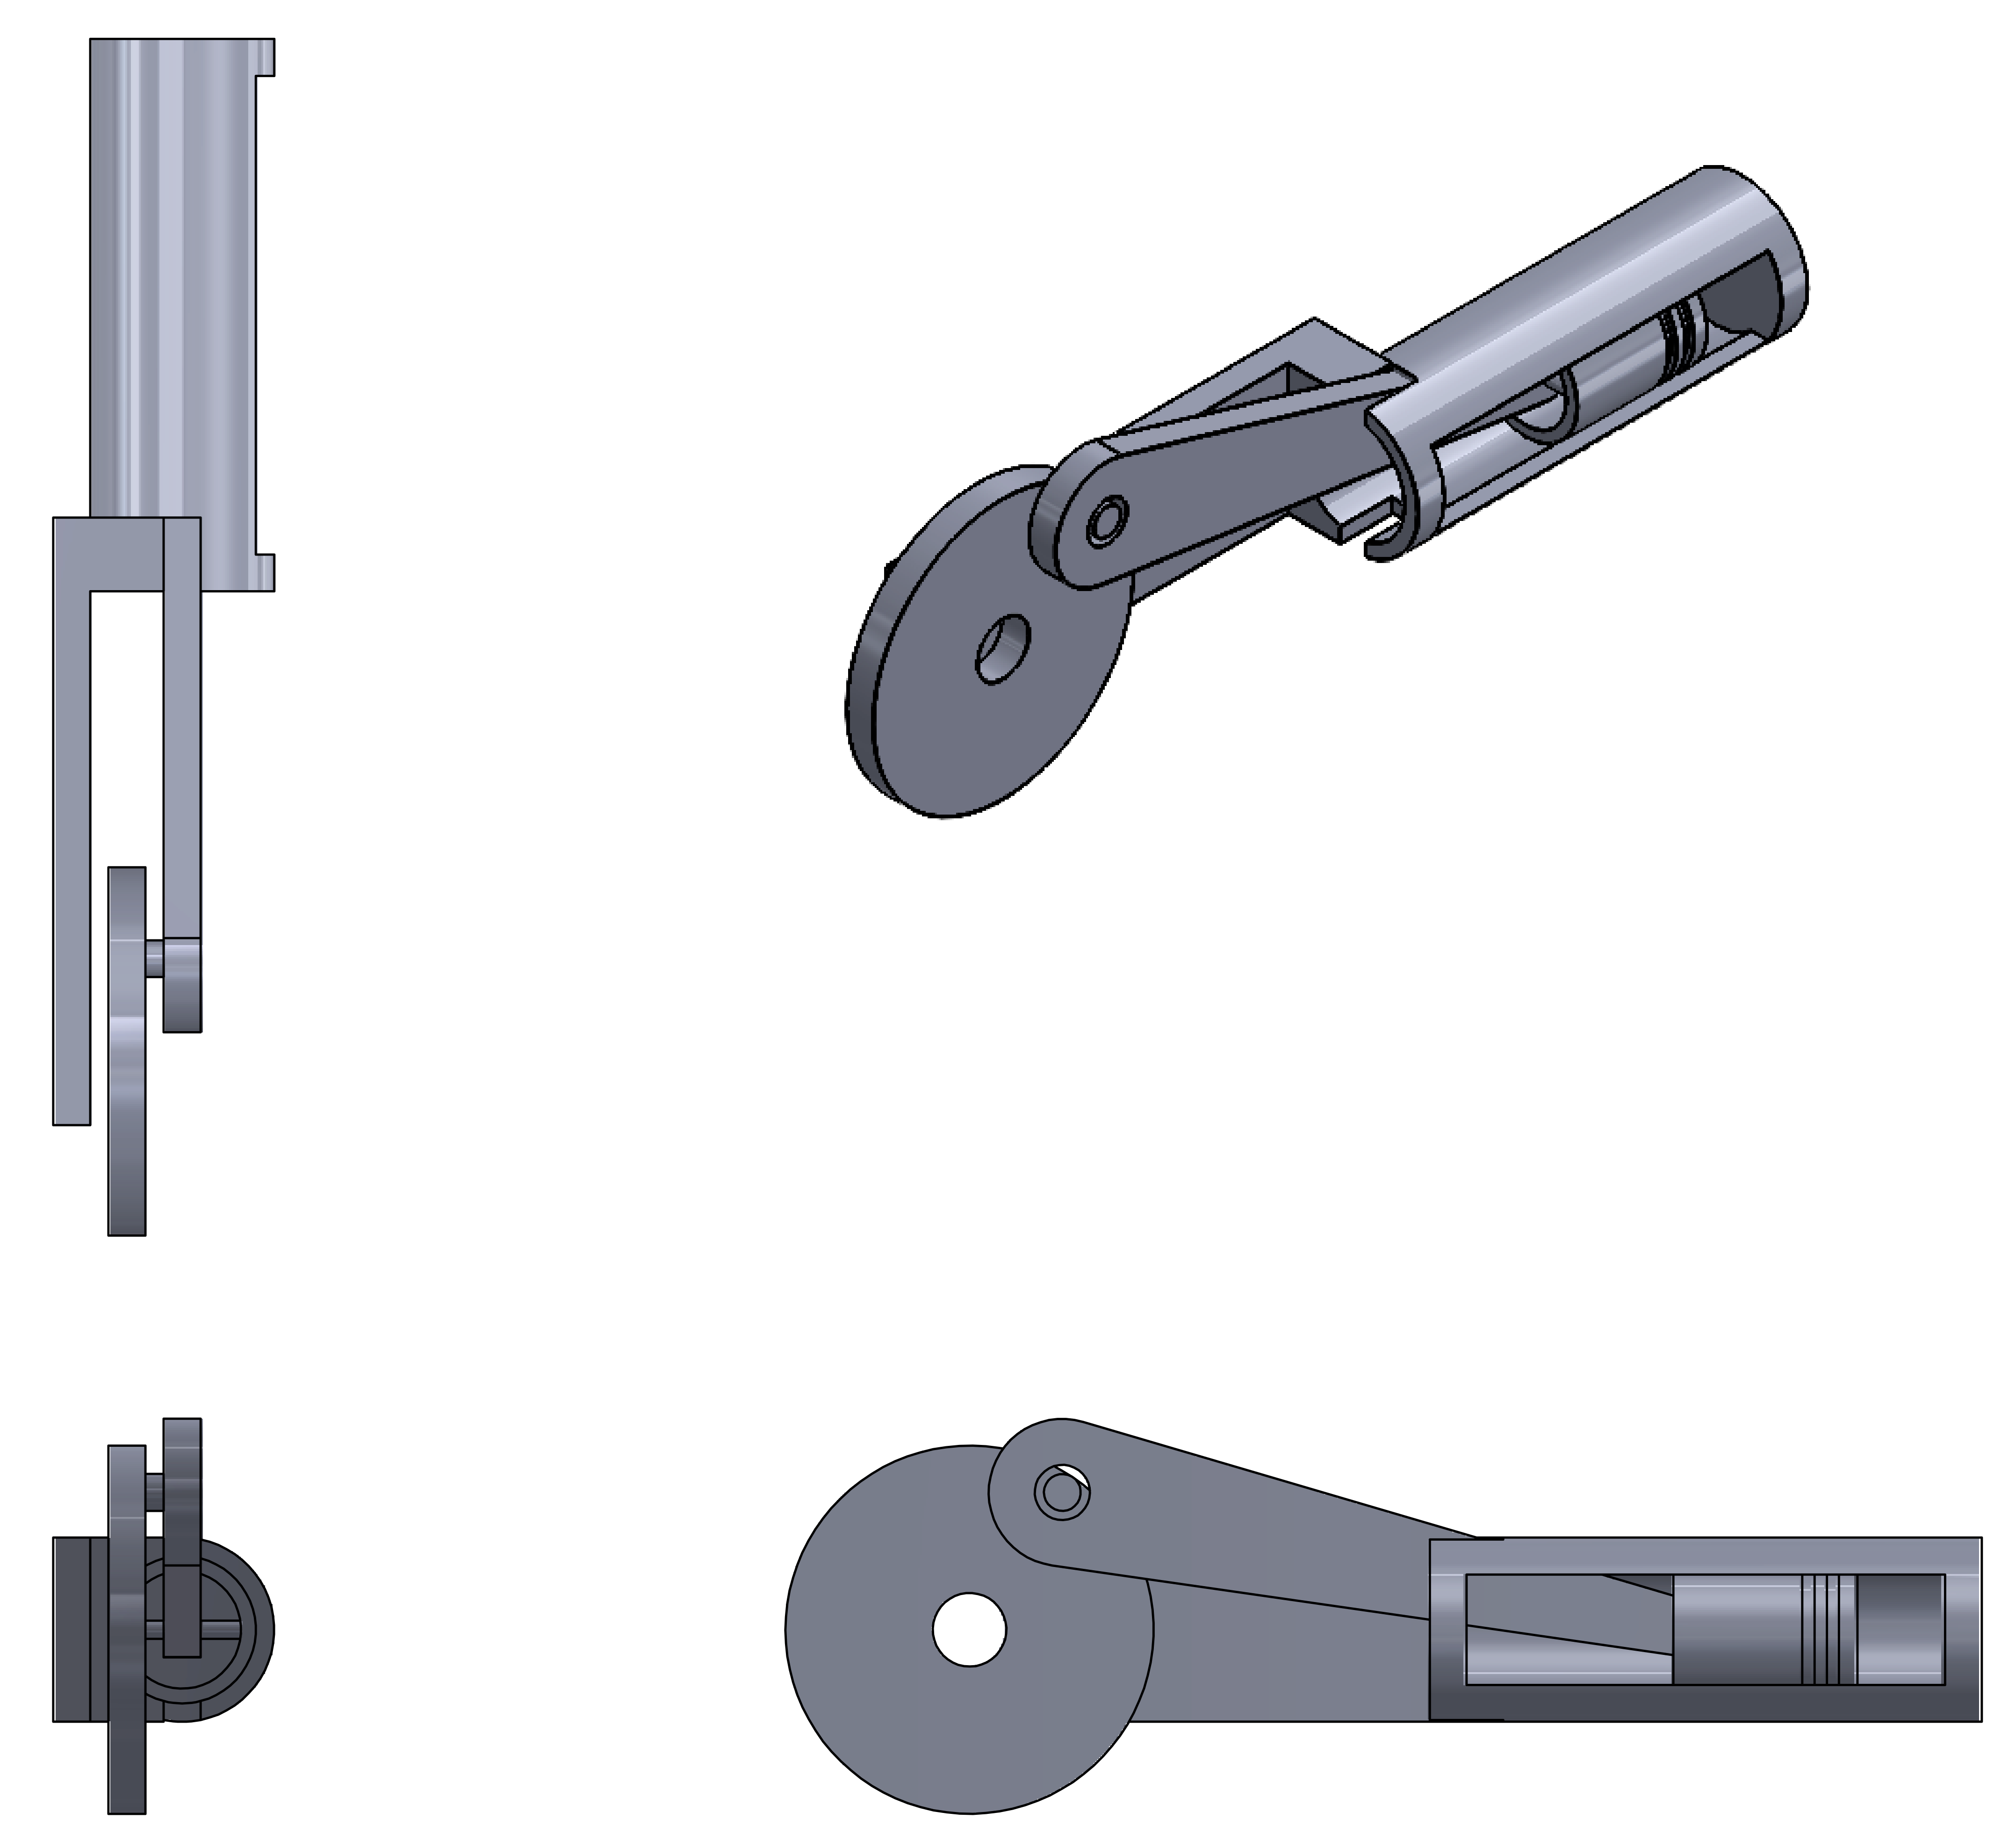
\includegraphics[width=.67\linewidth]{images/2.png}  
  \caption{Train}
  \label{fig:3}
\end{figure}
\vspace{1mm}
\end{minipage}
\begin{minipage}[c]{.25\linewidth}
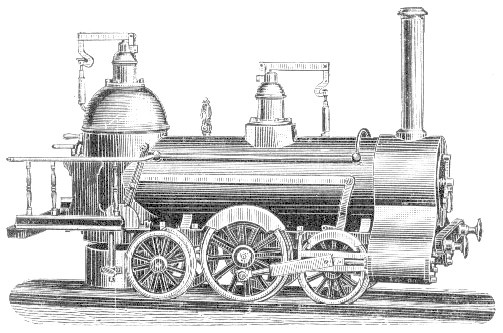
\includegraphics[width=\linewidth]{images/2b.jpg}
\end{minipage}
\noindent The first commercialized steam engine was developed by Thomas Savery in 1698 (over a millennium since steam engines were first created). Savery’s engines were used for pumping water out of mines. Steam engines would go on to play a crucial role in human progress and technological development. Steam turbines (which are a subset of steam engines) are very common today. Create the reciprocating piston assembly seen in \textit{Figure 2}. 

%problem 3
\textbf{P3}\\[0mm]
%\begin{minipage}[c]{.75\linewidth}
\begin{figure}[H]
  \centering
  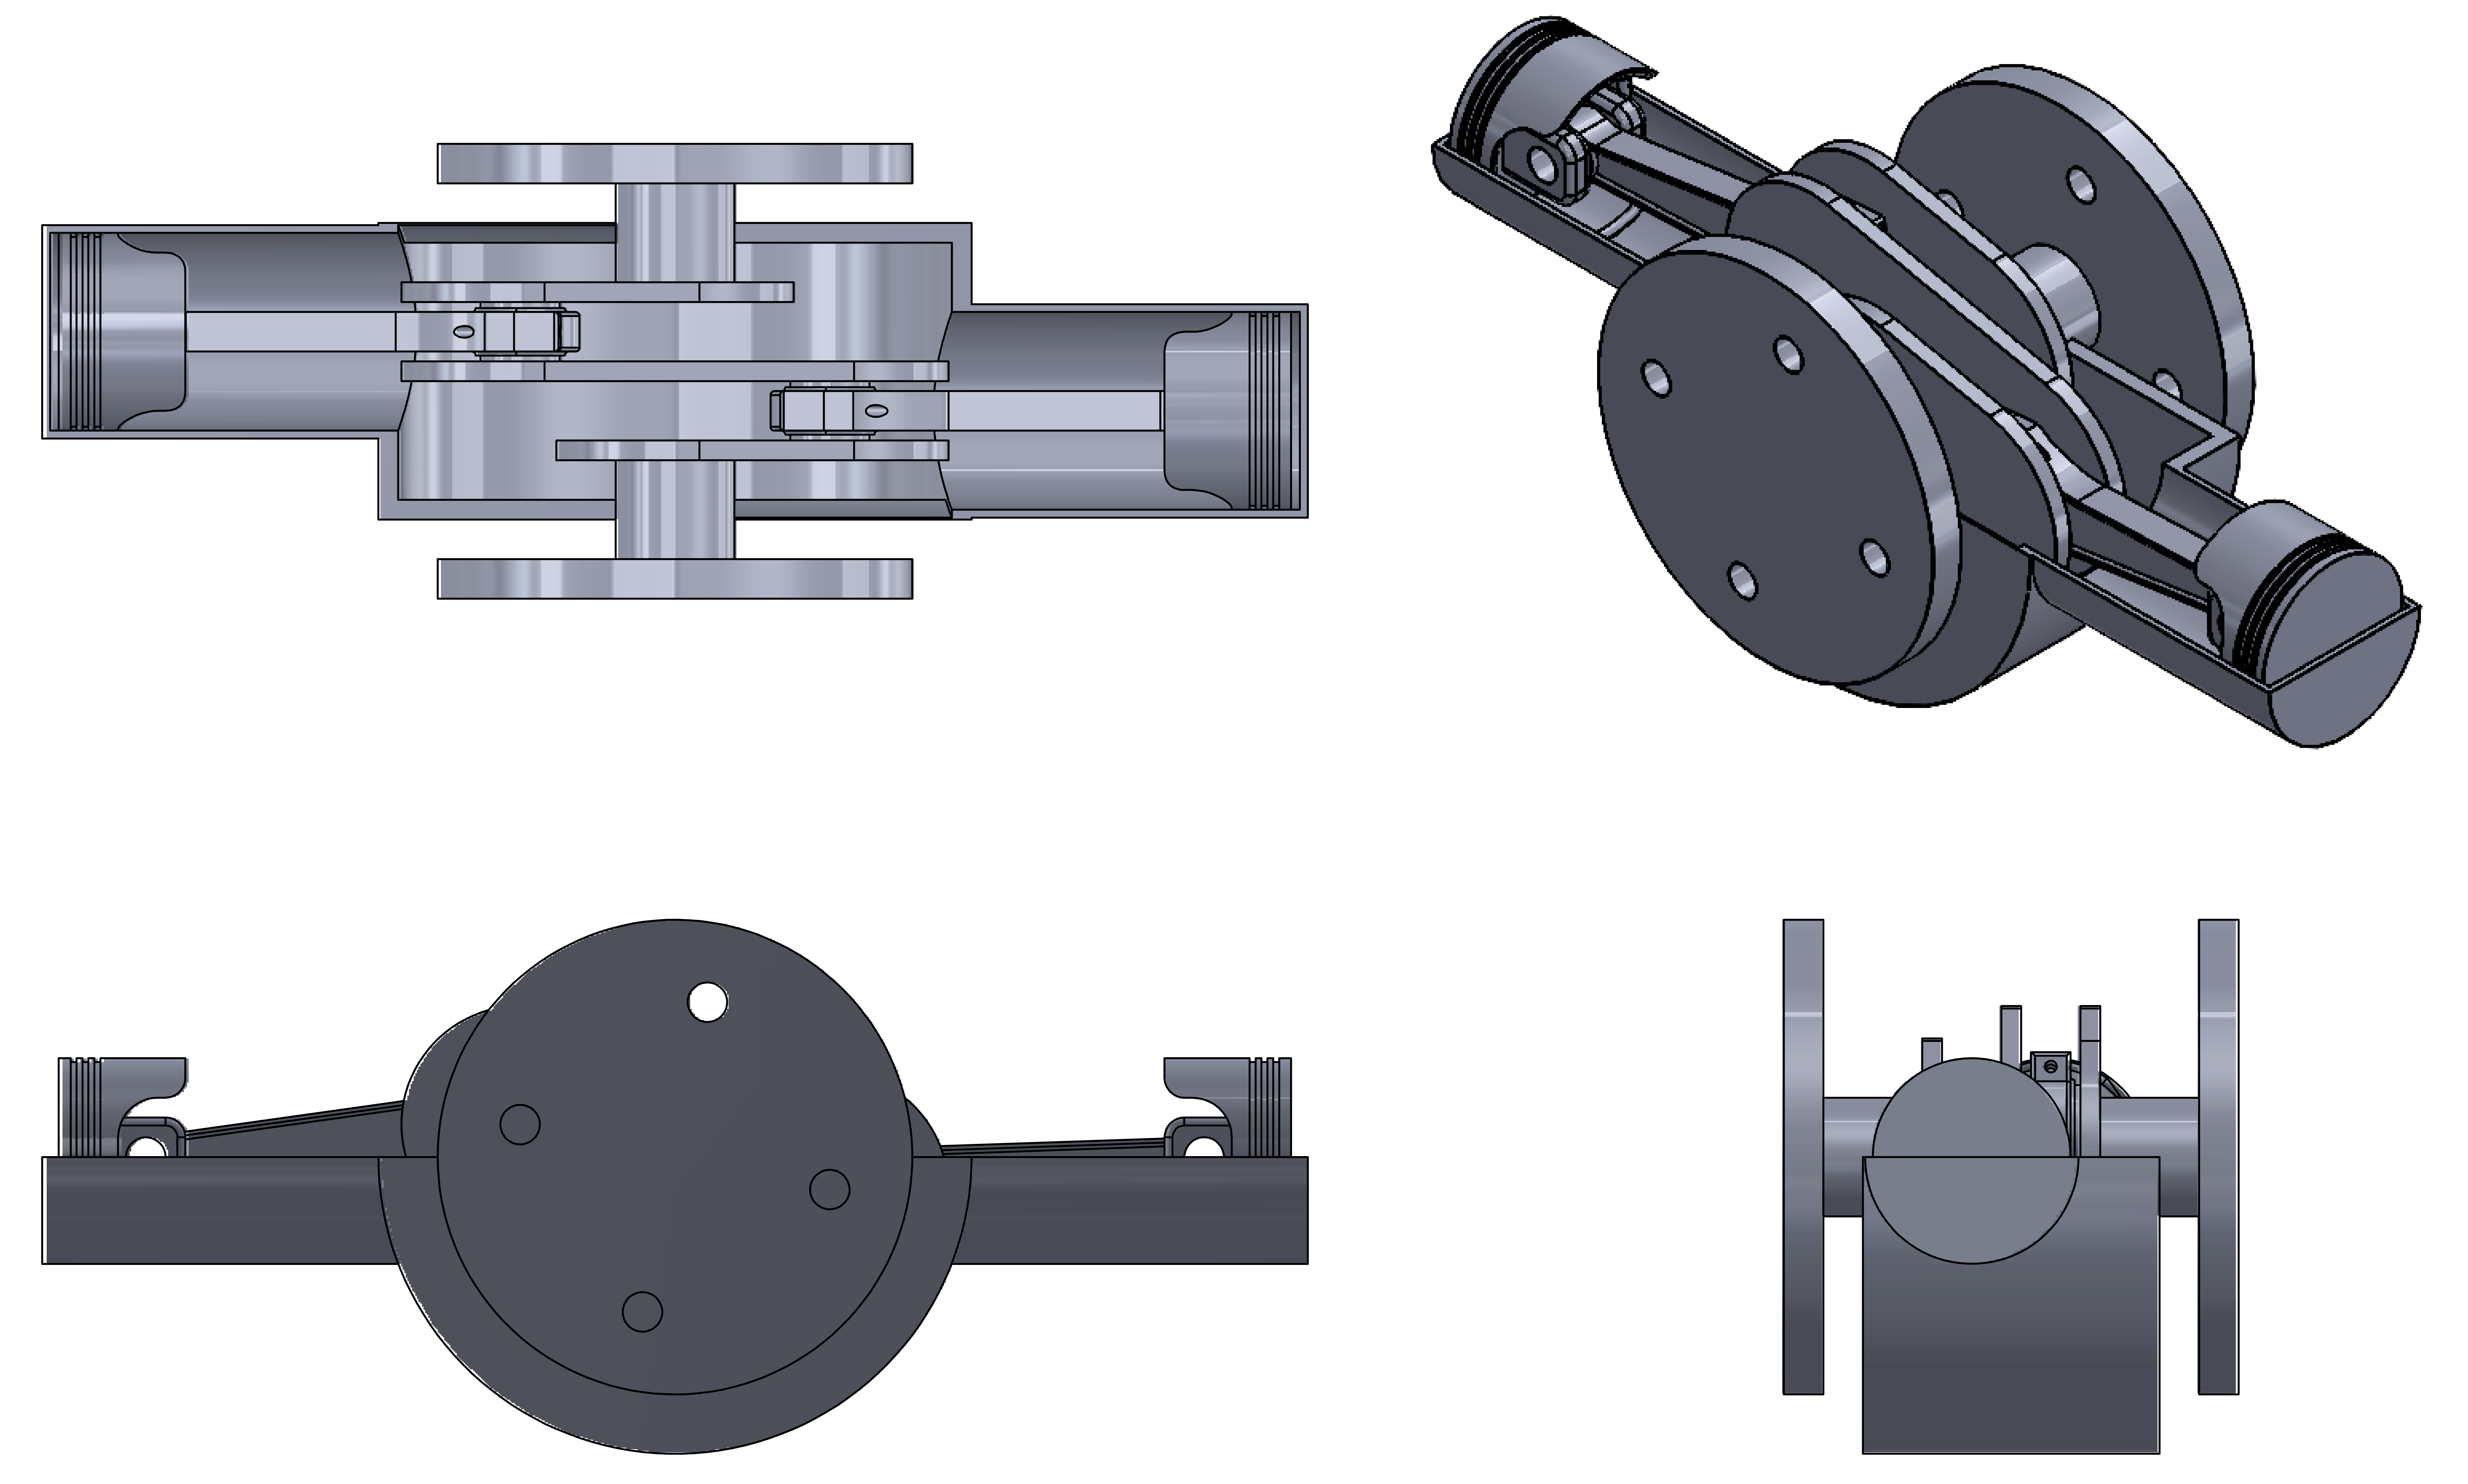
\includegraphics[width=.6\linewidth]{images/3.png}  %.9
  \caption{ICE}
  \label{fig:4}
\end{figure}
%\vspace{1mm}
%\end{minipage}
%\begin{minipage}[c]{.25\linewidth}
  \raggedleft{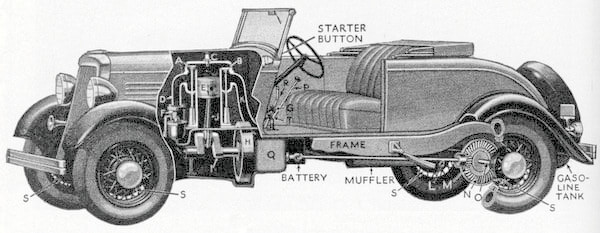
\includegraphics[width=.28\linewidth]{images/3b.jpg}}\\ %1
%\end{minipage}
\noindent\justify Internal combustion engines have revolutionized our world. George Brayton invented the first commercialized liquid-fuelled internal combustion engine in 1872. In 2019 globally 99\% of cars were powered by internal combustion engines. Please create the internal combustion engine assembly as seen in \textit{Figure 3}. 


%problem 4
\textbf{P4}\\[0mm]
\begin{minipage}[c]{.8\linewidth}
\begin{figure}[H]
  \centering
  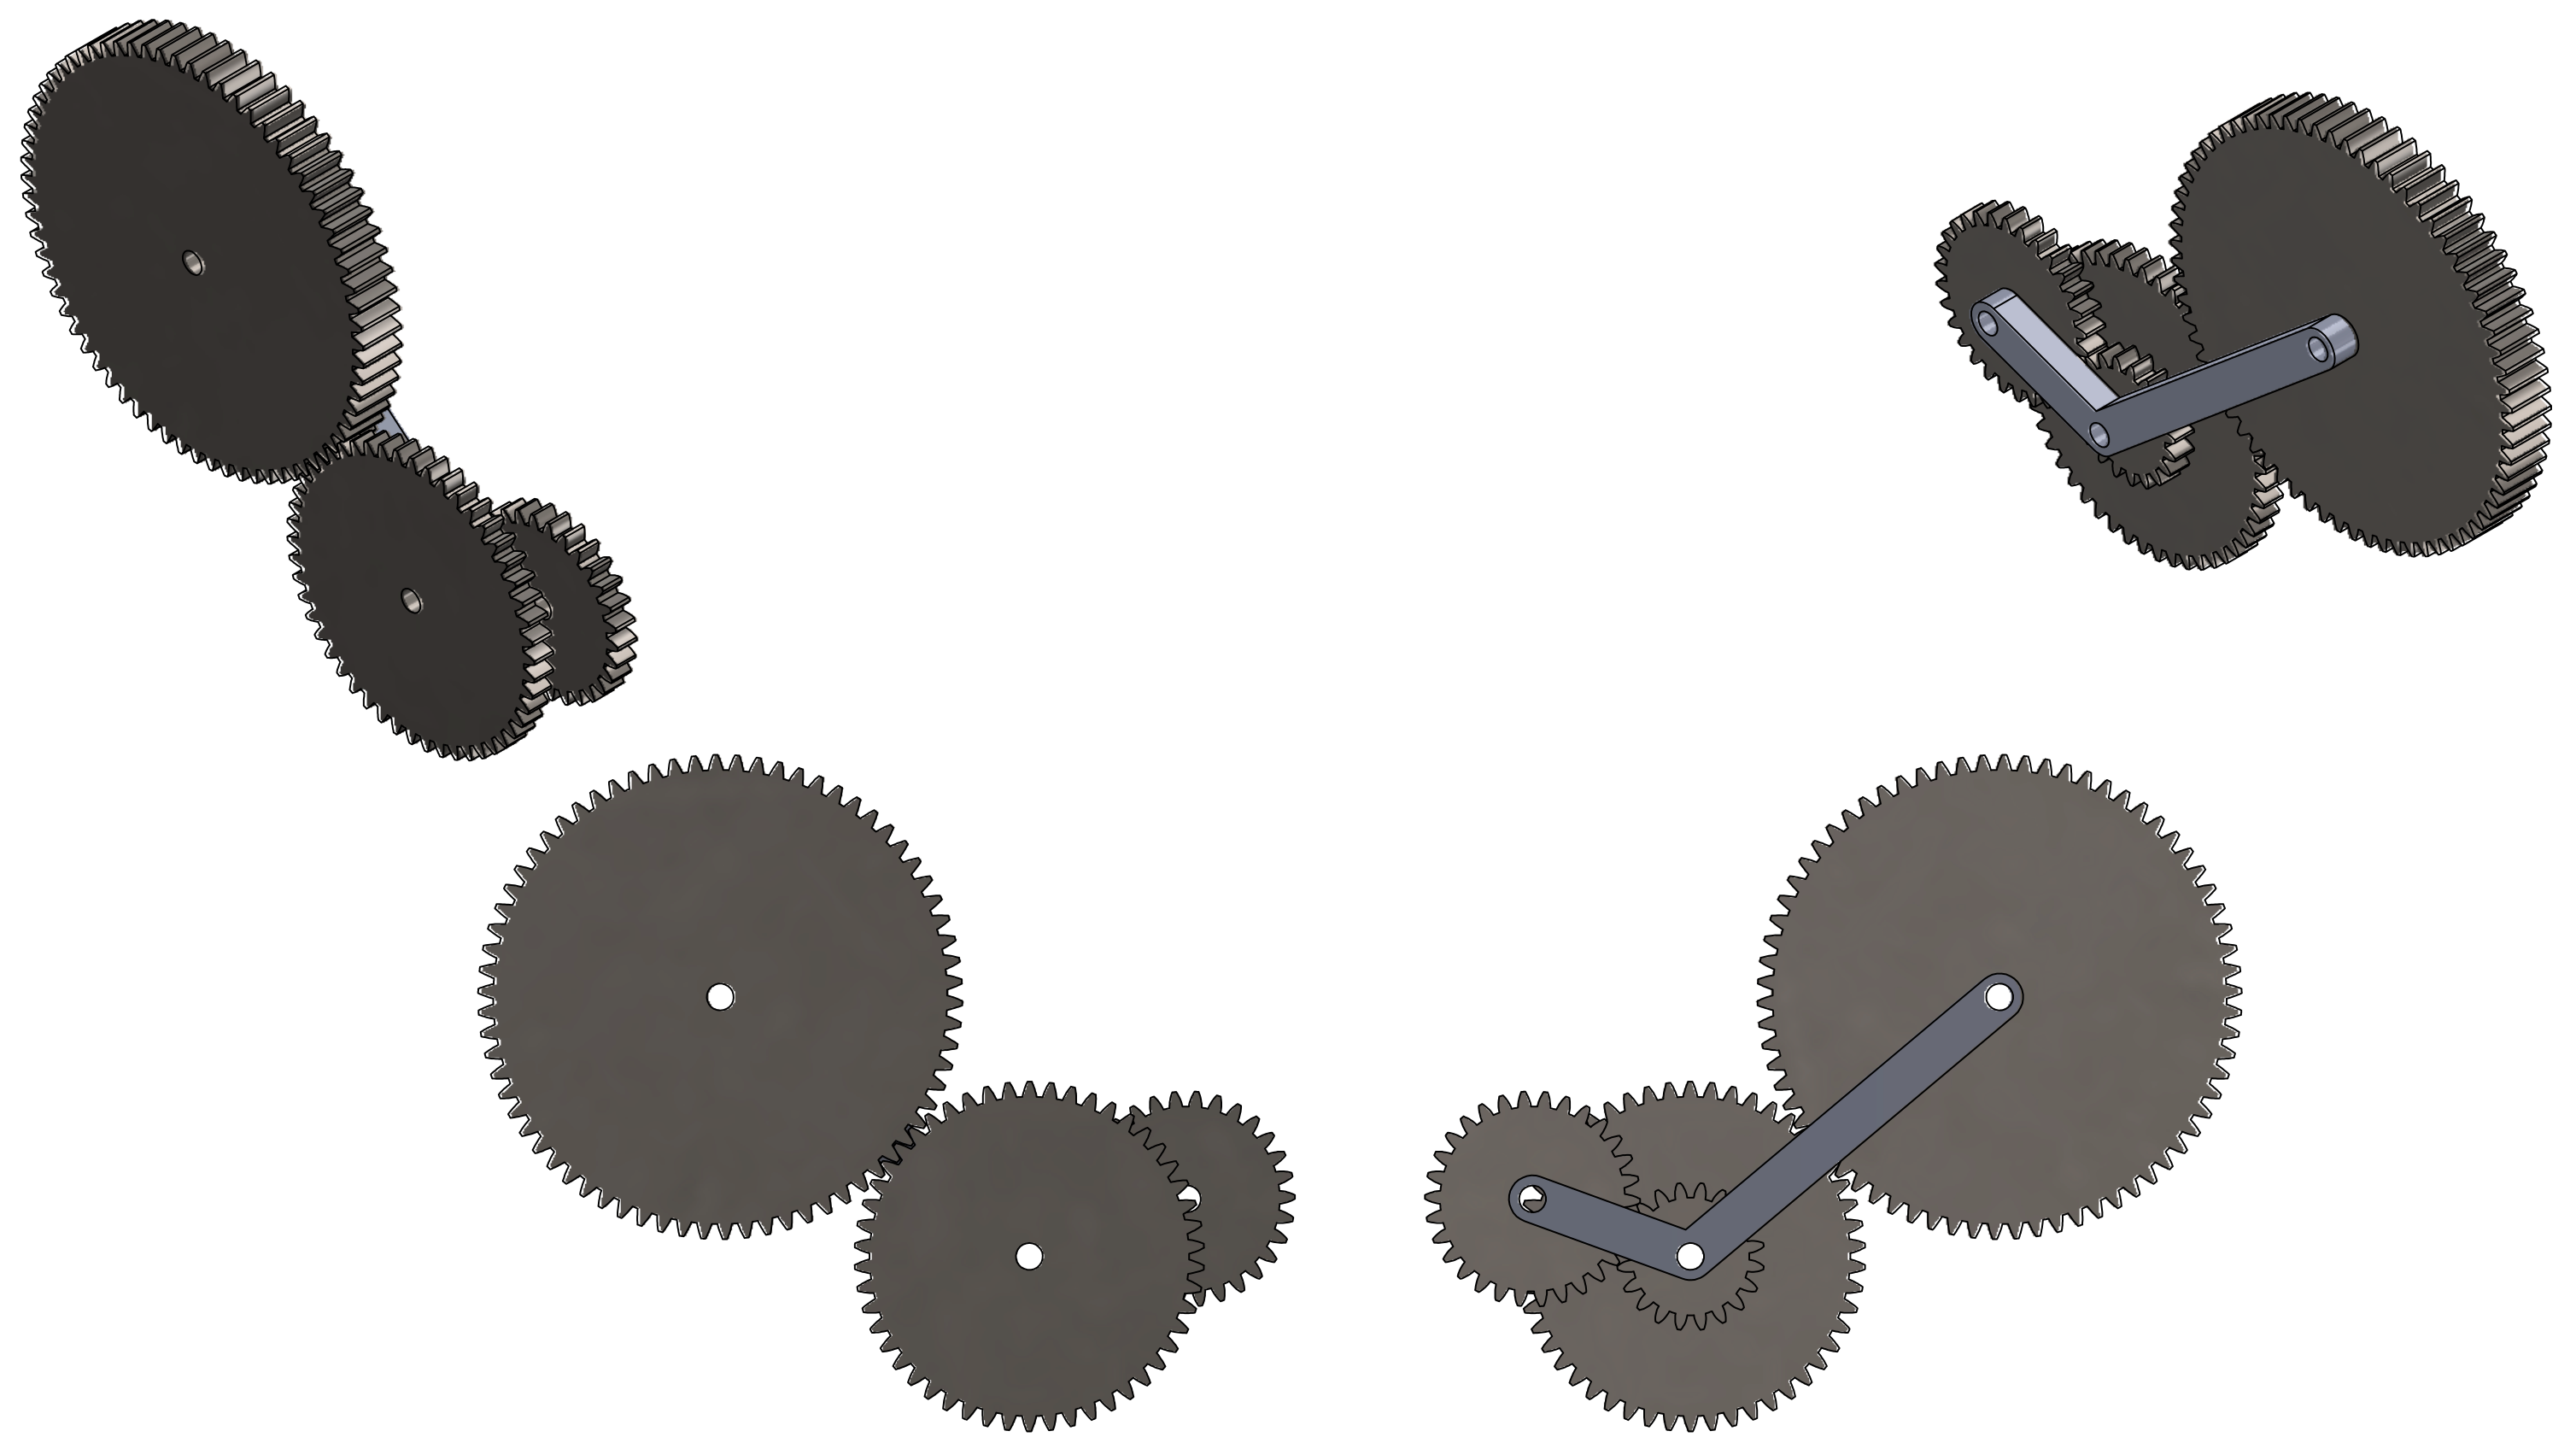
\includegraphics[width=\linewidth]{images/4.png} %.9  
  \caption{Gears}
  \label{fig:5}
\end{figure}
\vspace{1mm}
\end{minipage}
\begin{minipage}[c]{.2\linewidth}
\raggedleft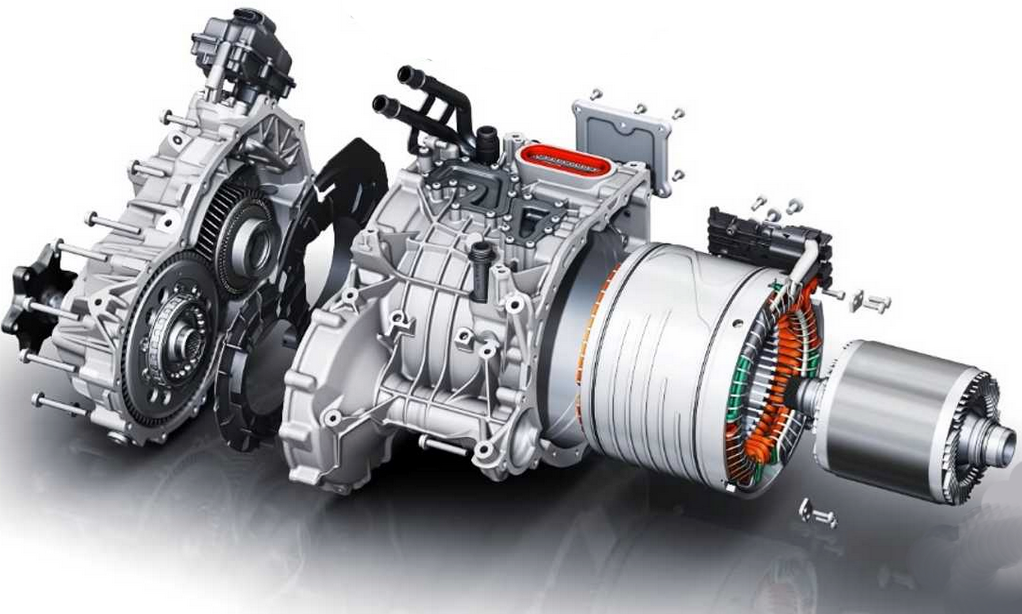
\includegraphics[width=1.2\linewidth]{images/4b.png} % 1.2
\hspace{5mm}
\end{minipage}
\noindent \\Electric motors have a number of advantages over internal combustion engines. The wide range of speed at which electric motors can operate efficiently allows electric motors to power cars without transmissions. It is still common for the initial speed of an electric motor to be slowed down through a gear train, not unsimilar to the one seen in Figure 4. Please create the gear train seen in \textit{Figure 4}. The gears should be able to rotate properly wrt. each other.
\end{document}
